\documentclass[12pt,a4paper]{article}

\usepackage{graphicx}
\usepackage{amsmath}
\usepackage{geometry}
\usepackage{fancyhdr}

\geometry{margin=0.9in}

% Header & Footer
\pagestyle{fancy}
\fancyhf{}
\lhead{Digital Logic}
\rhead{COMETFWC054}
\cfoot{\thepage}

\begin{document}

\begin{center}
    
\includegraphics[width=2.5cm]{assets/logo.jpg} \\[0.3cm]
    
    \textbf{\large KESHAVA REDDY V} \\[0.1cm]
    \textbf{ID: COMETFWC054} \\[0.3cm]
    
    \textbf{\Large Gate Logic Circuit Analysis}
\end{center}

\vspace{0.3cm}

\section*{Question}

For any set of inputs $A$ and $B$, the following circuits give the same output $Q$, except one.  
Which one is it? (GATE PH 2010)

\vspace{0.3cm}

\begin{center}
    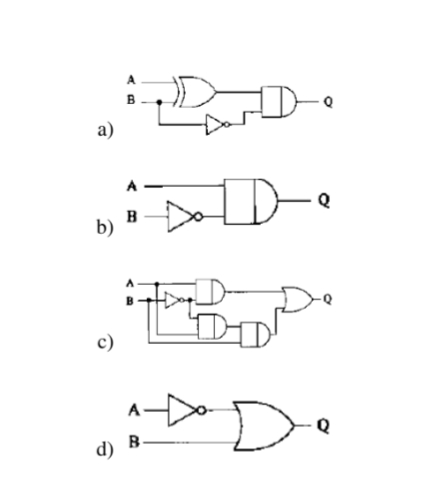
\includegraphics[width=0.8\textwidth]{pics/q41.jpg}
\end{center}

\section*{Solution}

We simplify each option using Boolean algebra.

\subsection*{Option (a)}

$$
Q = (A \oplus B)\overline{B}
$$

Since

$$
A \oplus B = A\overline{B} + \overline{A}B
$$

$$
Q = (A\overline{B} + \overline{A}B)\overline{B}
$$

$$
Q = A\overline{B}
$$

\subsection*{Option (b)}

$$
Q = A\overline{B}
$$

\subsection*{Option (c)}

After simplification,

$$
Q = A\overline{B}
$$

\subsection*{Option (d)}

$$
Q = \overline{A} + B
$$

This is not equal to $A\overline{B}$.

\vspace{0.3cm}

\begin{center}
\fbox{\large \textbf{Final Answer: Option (d) is different}}
\end{center}

\end{document}
